\documentclass[10pt]{article}

% Specify the margins and text size.
\setlength{\textwidth}{6.8in}
\setlength{\textheight}{9.5in}
\setlength{\oddsidemargin}{0pt}
\setlength{\evensidemargin}{0pt}
\setlength{\topmargin}{0pt}
\setlength{\hoffset}{-.1in}
\setlength{\voffset}{-1in}

\setlength{\parskip}{5pt}
\setlength{\parindent}{0pt}

% Load some fonts and symbol packages
\usepackage{latexsym}
\usepackage{pifont}       % contains 'star' symbol for counterinsurgency handbook title
\usepackage{yfonts} 
\usepackage{amsmath}
\usepackage{amsfonts}

\usepackage{graphicx}     % actually, this is loaded by pstricks
\usepackage[T1]{fontenc}
\usepackage{ifthen}
\usepackage{pstricks,pst-grad,pst-text,pst-node,multido,pst-plot,calc,pst-3dplot}
%\usepackage[all]{xy}
%\usepackage{animate}

% The hyperref package inserts links into the pdf.
\definecolor{MyLinkColor}{rgb}{.1,.2,1}
\definecolor{MyCiteColor}{rgb}{.1,1,.2}
\definecolor{MyURLColor}{rgb}{.4,.4,.4}
\usepackage[backref=true,pagebackref=false,hyperindex,colorlinks=true,
  linkcolor=MyLinkColor,urlcolor=MyURLColor]{hyperref}


% The tweaklist package is something I found on the web.  It provides a simple interface
% for making changes to spacing used in the itemize and enumerate environments.  Comment
% this out if you don't care to use tweaklist.
\usepackage{tweaklist}
\renewcommand{\itemhook}{\setlength{\parskip}{2pt}\setlength{\parsep}%
{1pt}\setlength{\topsep}{0pt}\setlength{\itemsep}{0pt}}

\newcommand{\U}{\underline{\hspace{5pt}}}

\usepackage{listings}
\newcounter{EX}\setcounter{EX}{1}
\newcommand{\EXERCISE}{\arabic{EX}.\stepcounter{EX} }

\begin{document}
\pagestyle{empty}
\lstset{language=R, showspaces=false, showstringspaces=false}

\href{http://www.su.edu}{
\includegraphics[height=1.75cm]{sulogo.eps}}
\vspace{-1.69cm}

{\small
\hbox{\ }\hfill\begin{tabular}{cl}
& Math 207\\
& Introduction to Statistics\\
& %23 January 2012
\end{tabular}
}
\setlength{\baselineskip}{1.05\baselineskip}
\bigskip

\begin{center}
\textbf{\large  Using \texttt{R} to Plot Histograms}
\end{center}
\medskip


\newcommand{\SUBX}{\smallskip\hspace{10pt}}
\newcommand{\BSK}{\vspace{.14in}}

\EXERCISE \texttt{R} has many built-in data sets.  The \texttt{mtcars} data set 
includes information extracted from the 1974 \textit{Motor Trend} US magazine, 
including fuel consumption and 10 aspects of automobile design and performance 
for 32 automobiles (1973--74 models).  First, let's look at the data:

\texttt{ > mtcars}\par

Next, let's use plot the \lq number of gears\rq\ data in a histogram.\par

\texttt{ > hist(mtcars\$gear, 
probability=TRUE, breaks=c(2.5,3.5,4.5,5.5), main="Motor Trend Car Data",}
\hphantom{+ }\texttt{  xlab="Number of Gears", ylab="Percent", ylim=c(0,0.5))}\vspace{-9pt}

\begin{figure}[h]
\begin{center}
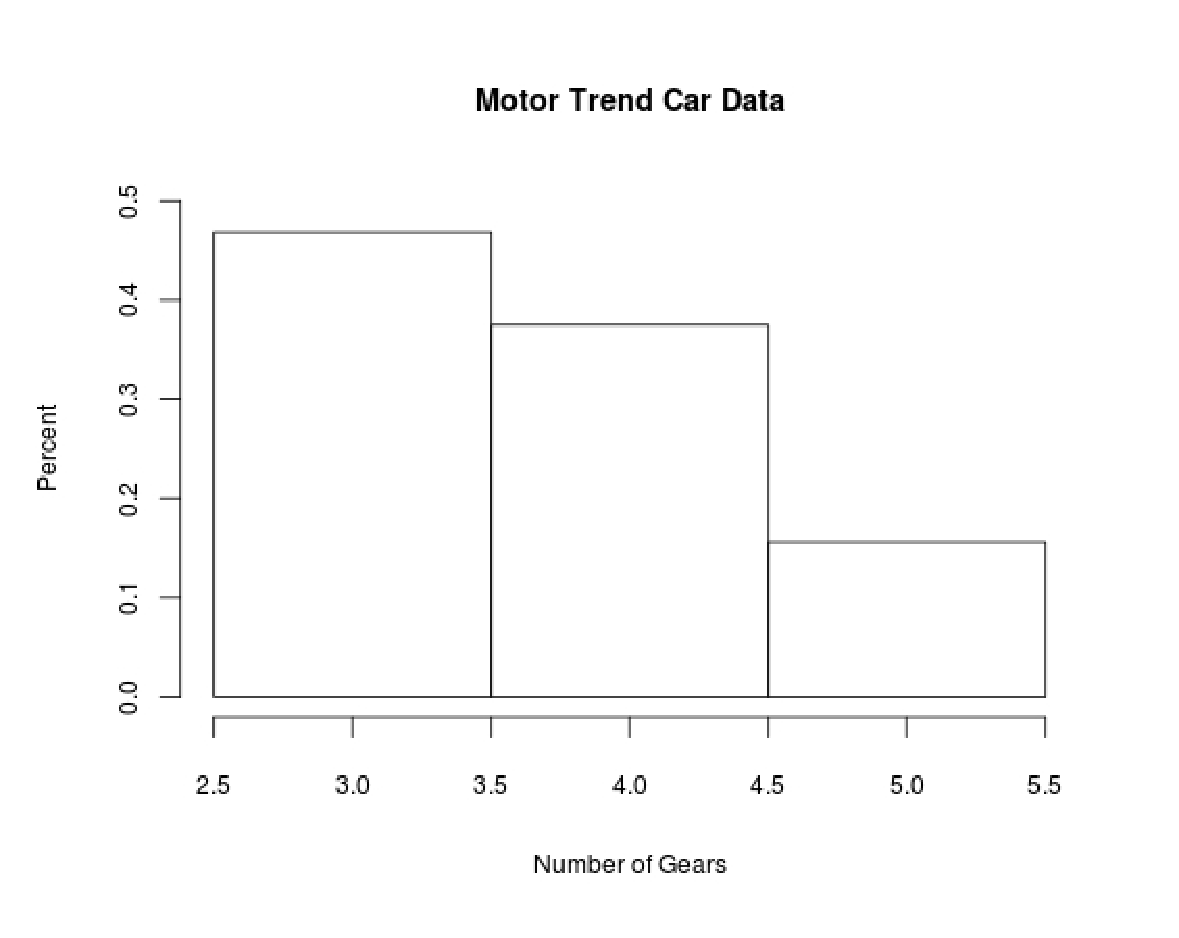
\includegraphics[height=2.9in, bb=0 16 550 360, clip]{MTcarsGears.eps}\vspace{-5pt}
\caption{\label{fig:gears}Histogram of Number of Gears based on \textit{Motor Trend} car data}\vspace{-1in}
\end{center}
\end{figure}
\vspace{.8in}

\EXERCISE  Use \texttt{R} to create a histogram of \texttt{mtcars\$mpg}, the mileage data for
  several 1973 car models.  To make your plot change the \texttt{xlab} and \texttt{ylab}
values from the ones in the previous exercise and delete the \texttt{breaks} option.
% hist(mtcars$mpg,probability=TRUE,xlab="Mileage", main="Motor Trend Car Data", 
% ylab="Percent",ylim=c(0,0.1))


\texttt{ > hist(mtcars\$mpg, probability=TRUE, main="Motor Trend Car Data",}
\hphantom{+ }\texttt{  xlab="Miles per Gallon", ylab="Percent", ylim=c(0,0.5))}


\EXERCISE  Use \texttt{R} to create a histogram of \texttt{mtcars\$am}, the transmission
  types for  several 1973 car models.  \par

\texttt{ > hist(mtcars\$am, probability=TRUE, main="Motor Trend Car Data", axes=FALSE,}\\
\hphantom{+ }\texttt{  xlab="Number of Gears", ylab="Percent")}\par
\texttt{ > axis(1, at=0:1, lab=c("Automatic", "Manual"))}\par
\texttt{ > axis(2, seq(0, 0.6, by=0.10))}\par
\medskip

\EXERCISE Pie charts are another way to illustrate data distributions.  
These are not 
recommended by some texts or in the \texttt{R} documentation.  
Here is an example of how
to create them, however.

\texttt{ > slices <- c(10, 12,4, 16, 8)}\vspace{-2pt}

\texttt{ > mylabels <- c("US", "UK", "Australia", "Germany", "France")}\vspace{-2pt}

\texttt{ > pie(slices, labels = mylabels, main="Pie Chart of Countries")}

\vfill
\eject

\end{document}

